\documentclass[10pt]{article}\usepackage[]{graphicx}\usepackage[]{color}
% maxwidth is the original width if it is less than linewidth
% otherwise use linewidth (to make sure the graphics do not exceed the margin)
\makeatletter
\def\maxwidth{ %
  \ifdim\Gin@nat@width>\linewidth
    \linewidth
  \else
    \Gin@nat@width
  \fi
}
\makeatother

\definecolor{fgcolor}{rgb}{0.345, 0.345, 0.345}
\newcommand{\hlnum}[1]{\textcolor[rgb]{0.686,0.059,0.569}{#1}}%
\newcommand{\hlstr}[1]{\textcolor[rgb]{0.192,0.494,0.8}{#1}}%
\newcommand{\hlcom}[1]{\textcolor[rgb]{0.678,0.584,0.686}{\textit{#1}}}%
\newcommand{\hlopt}[1]{\textcolor[rgb]{0,0,0}{#1}}%
\newcommand{\hlstd}[1]{\textcolor[rgb]{0.345,0.345,0.345}{#1}}%
\newcommand{\hlkwa}[1]{\textcolor[rgb]{0.161,0.373,0.58}{\textbf{#1}}}%
\newcommand{\hlkwb}[1]{\textcolor[rgb]{0.69,0.353,0.396}{#1}}%
\newcommand{\hlkwc}[1]{\textcolor[rgb]{0.333,0.667,0.333}{#1}}%
\newcommand{\hlkwd}[1]{\textcolor[rgb]{0.737,0.353,0.396}{\textbf{#1}}}%
\let\hlipl\hlkwb

\usepackage{framed}
\makeatletter
\newenvironment{kframe}{%
 \def\at@end@of@kframe{}%
 \ifinner\ifhmode%
  \def\at@end@of@kframe{\end{minipage}}%
  \begin{minipage}{\columnwidth}%
 \fi\fi%
 \def\FrameCommand##1{\hskip\@totalleftmargin \hskip-\fboxsep
 \colorbox{shadecolor}{##1}\hskip-\fboxsep
     % There is no \\@totalrightmargin, so:
     \hskip-\linewidth \hskip-\@totalleftmargin \hskip\columnwidth}%
 \MakeFramed {\advance\hsize-\width
   \@totalleftmargin\z@ \linewidth\hsize
   \@setminipage}}%
 {\par\unskip\endMakeFramed%
 \at@end@of@kframe}
\makeatother

\definecolor{shadecolor}{rgb}{.97, .97, .97}
\definecolor{messagecolor}{rgb}{0, 0, 0}
\definecolor{warningcolor}{rgb}{1, 0, 1}
\definecolor{errorcolor}{rgb}{1, 0, 0}
\newenvironment{knitrout}{}{} % an empty environment to be redefined in TeX

\usepackage{alltt}
\usepackage{graphicx, verbatim}
\usepackage{amsmath}
\usepackage{amssymb}
\usepackage{amscd}
\usepackage{lipsum}
\usepackage{blindtext}
\usepackage{todonotes}
\usepackage[tableposition=top]{caption}
\usepackage{ifthen}
\usepackage[utf8]{inputenc}
\usepackage{graphicx}
\usepackage{caption}
\setlength{\textwidth}{6.5in} 
\setlength{\textheight}{9in}
\setlength{\oddsidemargin}{0in} 
\setlength{\evensidemargin}{0in}
\setlength{\topmargin}{-1.5cm}
\setlength{\parindent}{0cm}
\usepackage{setspace}
\usepackage{float}
\usepackage{amssymb}
\usepackage[utf8]{inputenc}
\usepackage{fancyhdr}
\usepackage{tabularx}
\usepackage{soul}

\usepackage{hyperref}
\hypersetup{
  colorlinks   = true, %Colours links instead of ugly boxes
  urlcolor     = blue, %Colour for external hyperlinks
  linkcolor    = blue, %Colour of internal links
  citecolor   = red %Colour of citations
}

\usepackage[backend=biber ,sorting=none]{biblatex}
\bibliography{references}
\begin{filecontents*}{references.bib}
\end{filecontents*}


%\fancyhf{}
\rfoot{Group 2 \thepage}
\singlespacing
\usepackage[affil-it]{authblk} 
\usepackage{etoolbox}
\usepackage{lmodern}

% \makeatletter
% \renewcommand{\maketitle}{\bgroup\setlength{\parindent}{16pt}
% \begin{flushleft}
%   \textbf{\@title}
% 
%   \@author
% \end{flushleft}\egroup
% }

%\renewcommand\Authfont{\fontsize{14}{18.4}\selectfont}
%\makeatother

% \pagestyle{fancy}
% \rfoot{Page \thepage}
 %\thispagestyle{empty}
\IfFileExists{upquote.sty}{\usepackage{upquote}}{}
\begin{document}


\title{\LARGE Plastic Pollution in Oceans  \\ Group 2 Report - CMM507}

\author{ALEXANDER RITCHIE, \textit{\href{1911218@rgu.ac.uk}{1911218@rgu.ac.uk}};\\ GEORGIOS ORFANAKIS, \textit{\href{1903446@rgu.ac.uk}{1903446@rgu.ac.uk}};\\ KAREN JEWELL, \textit{\href{1415410@rgu.ac.uk}{1415410@rgu.ac.uk}};\\ ROSHI SHRESTHA, \textit{\href{1903445@rgu.ac.uk}{1903445@rgu.ac.uk}};\\ STUART WATT, \textit{\href{1501869@rgu.ac.uk}{1501869@rgu.ac.uk}}}

\maketitle
% \begin{flushleft} \today \end{flushleft} 
\noindent\rule{16cm}{0.4pt}
%\underline{\hspace{3cm}
\ \\
%\thispagestyle{empty}

\section*{Objective}


\begin{itemize}
\item To understand the composition of plastic pollutants in the ocean
\item To understand the sources of plastic pollutants
\item To understand how plastic pollution gets distributed across the oceans
\end{itemize}

\section{Problem Statement}\label{statement}

H1 = The \% of plastic pollution remains constant over time.

H0 = The \% of plastic pollution does not remain constant over time.




\subsection{Overview}\label{over}

Marine pollution is a major global issue which impacts on environment, economy and human health. Although marine pollution is caused by many different materials, plastics consist of 60-80\% of the marine litter.\cite{DERRAIK2002} \cite{REISSER2013} \cite{BARBOZA2020}
\\
\\
Synthetic organic polymer derived from polymerisation of monomers extracted from oil and gas make up the plastics.\cite{DERRAIK2002} \cite{RIOS2007} The lightweight feature and its durability make it very suitable to make a range of products that we use in our everyday life.\cite{BARNES2009} \cite{SIVAN2011} These same features have been a major cause of pollution due to overuse and non-managed waste disposal system worldwide with plastic contributing to the 10\% of the waste generated worldwide.\cite{BARNES2009} Due to its buoyancy, plastic debris can be dispersed over long distances and they can persist for a long time. Although, plastic litter has been a major cause of marine pollution for a while, its seriousness has only been realised recently. Jambeck et al.,\cite{JAMBECK2015} reported that in 2010 alone, between 4.8 million to 12.7 million metric tons of plastics entered the ocean. Plastics are now everywhere in the marine environment and urgent action is required to mitigate this problem and reduce the harmful impact.\cite{RIOS2007} \cite{ROCHMAN2015}



\subsection{Motivation}\label{mot}

Impact on marine life
\\
\\
Plastics in ocean is one of the many forms of human impact that threatens marine life. There is still very little information available on the impact of plastic pollution on the ocean's ecosystem. Due to the realisation on impact of human on climate and environment, there has been a lot of awareness activities to reduce the impact of pollution. Ban on single use plastic bags are being applied to many countries in order to protect the environment. 
\\
\\
Over 700 marine wildlife species are affected due to entanglement in plastic ropes and materials and ingestion of plastics in the ocean.\cite{GALL2015} Over 340 species of marine animals were found to be entangled.\cite{KUHN2015} Reducing plastic waste is a major challenge worldwide. It is almost impossible to estimate the number of marine animals affected by marine pollution globally due to the vastness of the ocean. However, studies carried out on the gut contents of thousands of seabirds, found the significant increase in the ingestion of plastics during the 10-15 years interval.\cite{ROBARDS1995} This result might correlate to the rapid increase of plastic production and plastic use globally.  In a study carried out over fourteen years, Moser and Lee \cite{MOSER1992} found that more 50\% of the seabird species contained plastic particles in the gut which increased over time. This could be due the increase in plastic availability over time. 
\\
\\
Entanglement in plastic debris is another cause of marine life suffering. Discarded fishing gear and floating mastic masses in ocean are serious threat to marine animals. Some animals such as seals are attracted to the floating plastics where they get entangled and get suffocated. Harmful effect of litter on marine life has been reviewed extensively.\cite{GALL2015} \cite{KUHN2015} \cite{RYAN2015} \cite{WILLIAMS2019} Floating plastics over long distances can disperse alien species as well as some pathogens. Drifting plastic debris are also the source of alien species introduction and thus affecting the native marine biodiversity.\cite{GREGORY2009} \cite{KIESSLING2015} 
\\
\\
Impact on environment and human health
\\
\\
Plastic debris floating in the oceans and the littering the coastal areas are not a pleasant sight. Masses of plastic accumulation and discarded objects made from plastics are found everywhere nowadays. 
\\
\\
Over time plastic disintegrates into small microplastics which are easily consumed by fish and they enter the food chain. Plastics have been found in a third of fish caught in the UK which included the popular fishes such as cod, haddock and mackerel. Impact of plastic entering the human food chain and the effects of it are still to be studied.  Plastic toxicity and the occurrence of microplastics and nanoplastics in the water supply can also be a direct impact on human health in addition to the contamination in seafood.\cite{ROCHMAN2015} \cite{MARKIC2020}
\\
\\
Reducing plastic pollution has recently been a global aim. Research in plastic pollution in marine environment has played a big role in reducing it and raising awareness all over the world. In order to understand the plastic pollution in marine environments and its effect in long term, it is essential to keep collecting data on patterns of marine debris around the world. Effective monitoring of plastic debris is very essential in order to reduce the abundance of plastic debris everywhere. In addition, monitoring the type, frequency and the source of the litter is also important for prevention initiative of marine pollution. Most of the monitoring are done by surveys looking at frequencies of beach litter collected by organisations and volunteers.\cite{COE1997} Most abundant litter can be found close to urban areas where beach visitor numbers are higher.\cite{GARRITY1993} 






\subsection{Objectives }\label{obj}

The main objectives of this project can be outlined as follows: 



\pagebreak
\section{Research}\label{research}

Things we found

Sources of pollution: 10 river dataset, 50km2 coastline dataset, pollution density and body of water dataset....

\pagebreak
\section {Methods}\label{methods}

This paper is conducted using secondary data collection methods only. The authors did not collect or create any new data using primary methods.


\subsection{Dataset Description}\label{dataset}

\hl{data dictionary is probably better as a table than a list.}
\hl{Can we also add to this information of how the data is entered e.g. optional/mandatory fields, free-text or dropdown fields. The use of IDs suggest these are option fields with lookup tables somewhere.}

\begin{itemize}
%\Where the dataset came from; How it is constructed: multiple csv files by year; A description of what it is, what's in it and what it represents; Problems with the dataset: Missing data; data anomalies (lat/long values don't match named regions)

\item The data was taken from  \textit{\href{http://marinedebris.engr.uga.edu/newmap/}{marine debris tracker}} between 2010 till February 19th 2020. The time of 2010 was chosen as there was no data before that time.
\item The dataset was composed by combining the multiple csv files gathered from the marine debris tracker into a single set after this was done the date data type was renamed "Time". 
\item The dataset created from the combined csv files contain more than 360000 rows of data and consists of the folowing variables. 
  \begin{itemize}
  \item ListID is the ID code for the list
  \item ListName is the name of the list
  \item ItemID is the ID code given to the item of debris
  \item ItemName is the name we give to item of debris
  \item LogID is the ID code given to the location of the debris
  \item Latitude, Longitude and Altitude are the coordinates of the location where the observation was made
  \item Quantity is the number of pieces of debris in the observation.
  \item Error radius is the radius around the observation site within the error for reasonable doubt.
  \item Location is the area the observation of debris was made in.
  \item Description is the description of the area the debris was found in.
  \item MaterialID is the ID code of the material that the debris was composed of. 
  \item Material Description is the description given to the material that composes the debris.
  \item Time is the time that the observation was made. 
\item There were a number of problems with the dataset namely;
  \begin{itemize}
  \item There were a number of cases of missing data in the dataset. 
  \item data anomalies (lat/long values don't match named regions)
  \item 
  \end{itemize}
\end{itemize}
\end{itemize}

\subsection{Dataset Pre-processing}
%\Because of the features and concerns identified in the section above, we chose to transform the dataset in the following ways:reclassified some labels because variation was too high (there were too many labels); removed missing values; removed certain subsets; but kept certain subsets

Everything below is from Stuart's RNW file



\begin{knitrout}
\definecolor{shadecolor}{rgb}{0.969, 0.969, 0.969}\color{fgcolor}\begin{kframe}
\begin{verbatim}
## [1] "Location"    "Description"
\end{verbatim}
\end{kframe}
\end{knitrout}
The following actions were performed on the dataset:

\"ListID\" and \"ListName\" were found to be redundant and removed. \hl{can we remove ItemID and MaterialID also since we have the descriptions?}\\
\\
Nulls found in ItemName and Description.\\ 
\hl{this means every entry has a material at least? why? could be a required field? that would explain why some entries are rubbish if people are forced to pick a category}
\hl{it is also worth discussing the merits of dropdown entries: standardises input but forces a value where none might be appropriate, or a default it selected?}
\\
\hl{Stuart: Yes, it is a required field. I checked on the mobile app and you select a item type from different material sections. Note however that there is a material type \emph{Other Items} which contains the items \emph{Other} and \emph{Test Item}. Therefore users are able to categorise an item as other if it is not appropriate for any other option on the list.}
\\
NAs removed \hl{not sure what is actually happening with the explicit\_na() piece for location?}\\
\\
\hl{Stuart: I used explicit\_na to replace missing values with an expliciet level name (like ``Missing'' or something similar). I think it was to remove warnings when I was plotting.}
\\
\hl{also maybe worth looking at: what's the significance of some of these itemIDs where the itemname is blank? It could be an item once that was then deleted or categorised retrospectively. Do a groupby ItemID and see if more than one material or item name turns up.}\\
\\
\hl{I was puzzled by this so I investigated it and found it is not in the source data. I found a coding bug further down in the code, where I make the stacked bar chart with proportions per month. I have fixed this, and now no ItemName values are blank. Sorry!}
\\
Unique values for each column: \hl{can we present these unique counts as a formatted table? I think it's interesting that 55 unique items can have \~8k descriptions}
\begin{knitrout}
\definecolor{shadecolor}{rgb}{0.969, 0.969, 0.969}\color{fgcolor}\begin{kframe}
\begin{verbatim}
##               ItemID             ItemName                LogID 
##                   55                   55               363368 
##             Latitude            Longitude             Altitude 
##               142707               136490               135214 
##             Quantity         Error Radius             Location 
##                  496                18374                 1458 
##          Description          Material ID Material Description 
##                 8494                    8                    8 
##                 Time 
##               248436
\end{verbatim}
\end{kframe}
\end{knitrout}

\subsection{Data Quality Issues: Classification}
The authors find that there are multiple instances of missclassified items. Where their descriptions appear to not match their material categorisation\\
Lets see if there are any "ItemNames" associated with more than one "Material Descriptions".
\begin{knitrout}
\definecolor{shadecolor}{rgb}{0.969, 0.969, 0.969}\color{fgcolor}\begin{kframe}
\begin{verbatim}
## # A tibble: 1 x 2
##   ItemName          n
##   <chr>         <int>
## 1 Rubber Gloves     2
\end{verbatim}
\end{kframe}
\end{knitrout}
So rubber gloves are associated with two material descriptions, but otherwise a one to many relationship exists between "Material Description" and "ItemName".
\begin{knitrout}
\definecolor{shadecolor}{rgb}{0.969, 0.969, 0.969}\color{fgcolor}\begin{kframe}
\begin{verbatim}
## # A tibble: 2 x 2
##   `Material Description` Quantity
##   <fct>                     <dbl>
## 1 PLASTIC                    2114
## 2 RUBBER                      155
\end{verbatim}
\end{kframe}
\end{knitrout}
It seems that most rubber gloves are classified as plastic rather than rubber.
\begin{knitrout}
\definecolor{shadecolor}{rgb}{0.969, 0.969, 0.969}\color{fgcolor}\begin{kframe}
\begin{verbatim}
## # A tibble: 33 x 3
##    `Material Description` ItemName     Description                              
##    <fct>                  <fct>        <chr>                                    
##  1 PLASTIC                Rubber Glov~ Found on wassaw island Oct. 21 with beac~
##  2 PLASTIC                Rubber Glov~ undefined                                
##  3 PLASTIC                Rubber Glov~ undefined                                
##  4 PLASTIC                Rubber Glov~ thermal                                  
##  5 PLASTIC                Rubber Glov~ Near water                               
##  6 PLASTIC                Rubber Glov~ Taste of Omaha Cleanup                   
##  7 PLASTIC                Rubber Glov~ Taste of Omaha Cleanup                   
##  8 PLASTIC                Rubber Glov~ 2 diff kinds                             
##  9 PLASTIC                Rubber Glov~ undefined                                
## 10 PLASTIC                Rubber Glov~ Latex                                    
## # ... with 23 more rows
\end{verbatim}
\end{kframe}
\end{knitrout}
All instances of rubber gloves with non-missing descriptions are categorised as plastic. We also see that the descriptions suggest that the categorisation may be innaccurate: the last two instances here have "Balloon" in the extra descriptions... why aren't they categorised as such?
\hl{another thing maybe worth looking at: all MATERIALS!=Plastic yet have the term "plastic" in the description. could further expand this to descriptions which have any of the material terms in them, but is not its own material. further explores the point about missclassified data.}





\subsection{Recategorisation}


After the issues with the dataset that were identified in the section above, it was decided that it would be best to transform the dataset in the following ways:
\begin{itemize}
\item reclassified some labels because variation was too high (there were too many labels)
\item The values of the missing data were removed.
\item It was decided that subsets that were not needed were removed while retaining the necessary subsets.
\end{itemize}

\begin{figure}[H] %start a figure
\begin{center}
\begin{knitrout}
\definecolor{shadecolor}{rgb}{0.969, 0.969, 0.969}\color{fgcolor}
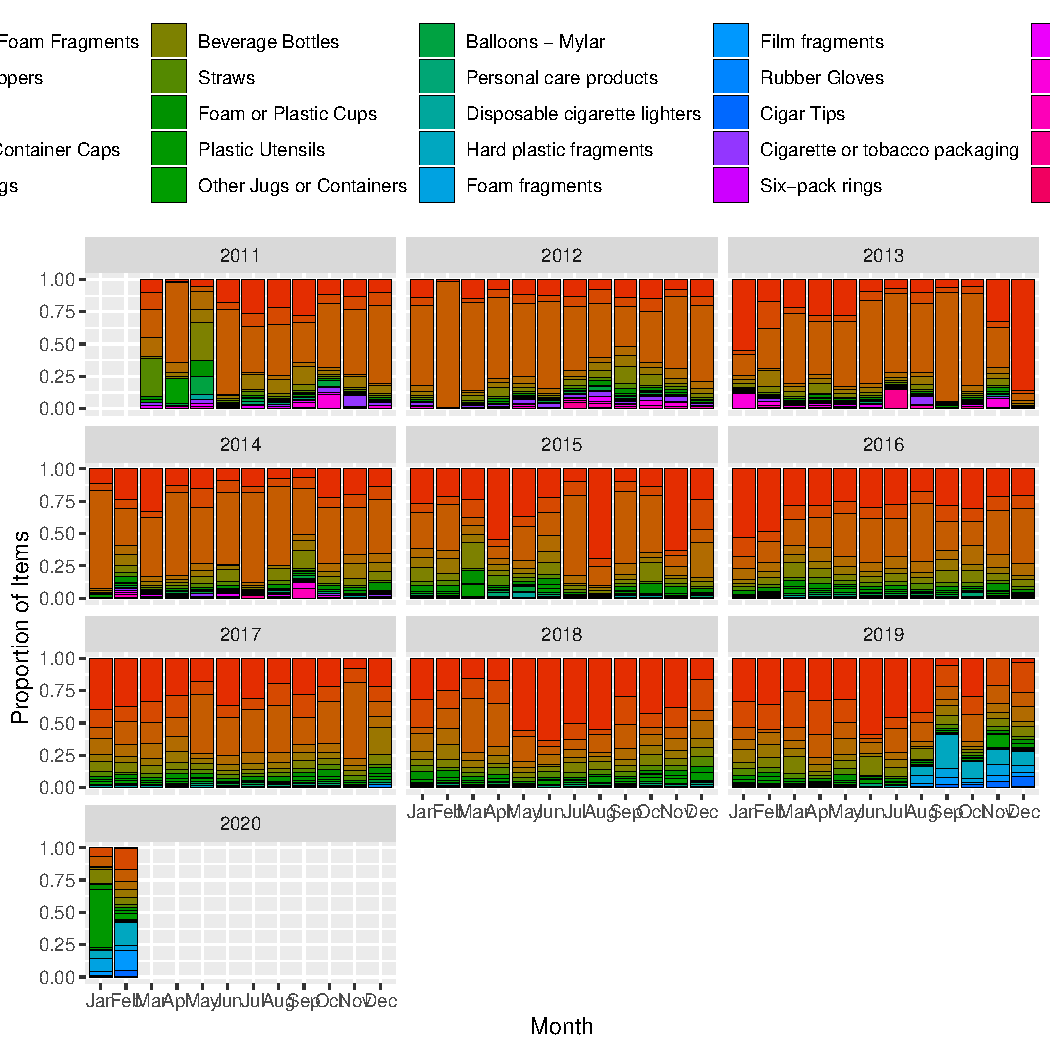
\includegraphics[width=\maxwidth]{figure/unnamed-chunk-7-1} 

\end{knitrout}
\caption {Debris by categorisation}
\label{figE}
\end {center}
\end {figure}





\begin{figure}[H] %start a figure
\begin{center}
\begin{knitrout}
\definecolor{shadecolor}{rgb}{0.969, 0.969, 0.969}\color{fgcolor}
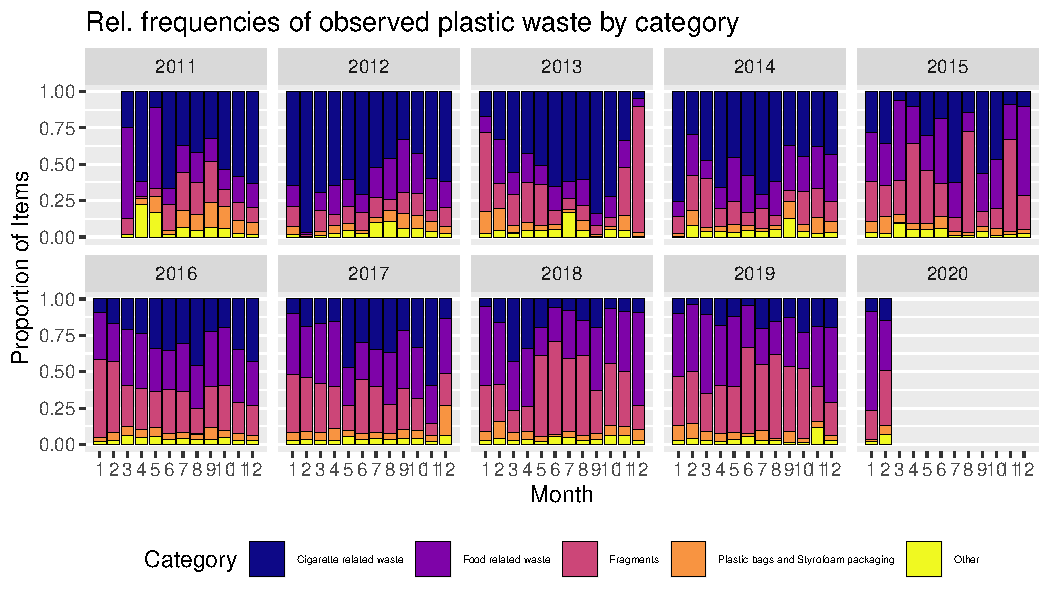
\includegraphics[width=\maxwidth]{figure/unnamed-chunk-8-1} 

\end{knitrout}
\caption {Recategorisation by year}
\label{figB}
\end {center}
\end {figure}



\pagebreak
\section{Exploration}

Here we describe the things we found... 

\subsection{Proportion Trends}
How pollutant proportions change over time.\\
\\
Cigarette butts proportions and raw counts decrease over time: possibly less people smoking, or moving to vaping\\
\\
General pollution count going down over time?\\
\\
Old pollutants fall away (cigarette butts) but new ones are introduced\\
\\
Question: Are observed plastic item proportions time invariant?\\
\\
\begin{figure}[H] %start a figure
\begin{center}
\begin{knitrout}
\definecolor{shadecolor}{rgb}{0.969, 0.969, 0.969}\color{fgcolor}
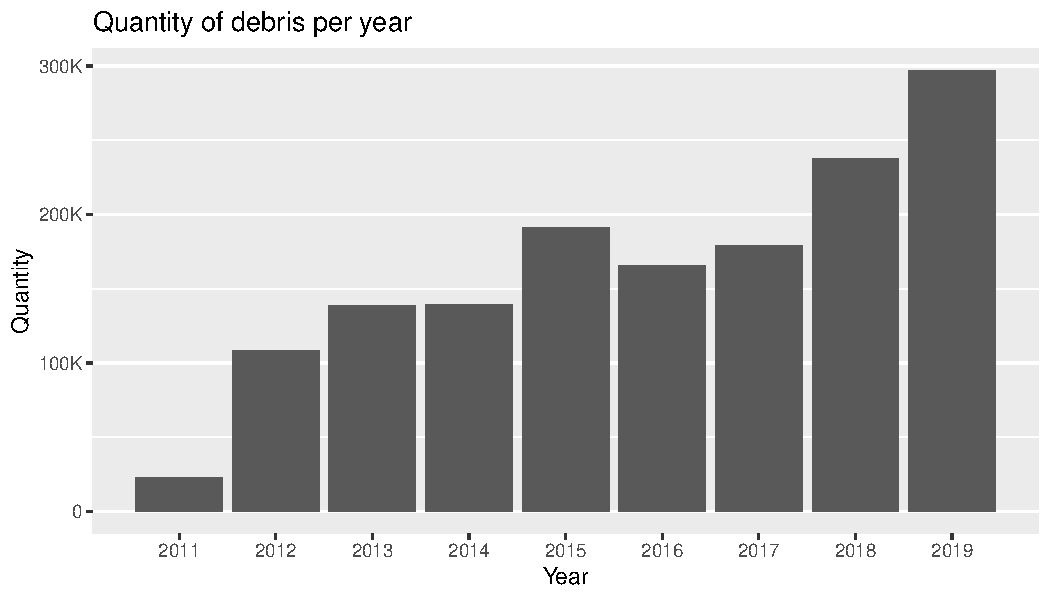
\includegraphics[width=\maxwidth]{figure/unnamed-chunk-9-1} 

\end{knitrout}
\caption {Trend of debris observered}
\label{figD}
\end {center}
\end {figure}
\hl{this chart needs to size down}



\begin{figure}[H] %start a figure
\begin{center}
\begin{knitrout}
\definecolor{shadecolor}{rgb}{0.969, 0.969, 0.969}\color{fgcolor}
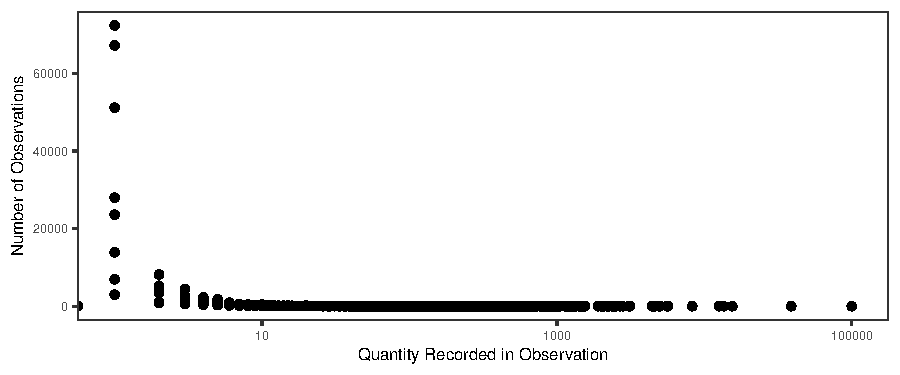
\includegraphics[width=\maxwidth]{figure/unnamed-chunk-10-1} 

\end{knitrout}
\caption {Observations of plastic debris v all debris}
\label{figF}
\end {center}
\end {figure}
\hl{this chart needs to size down}



\subsection {Distribution of observed debris:}

MaterialQuantities\\

\begin{figure}[H] %start a figure
\begin{center}
\begin{knitrout}
\definecolor{shadecolor}{rgb}{0.969, 0.969, 0.969}\color{fgcolor}
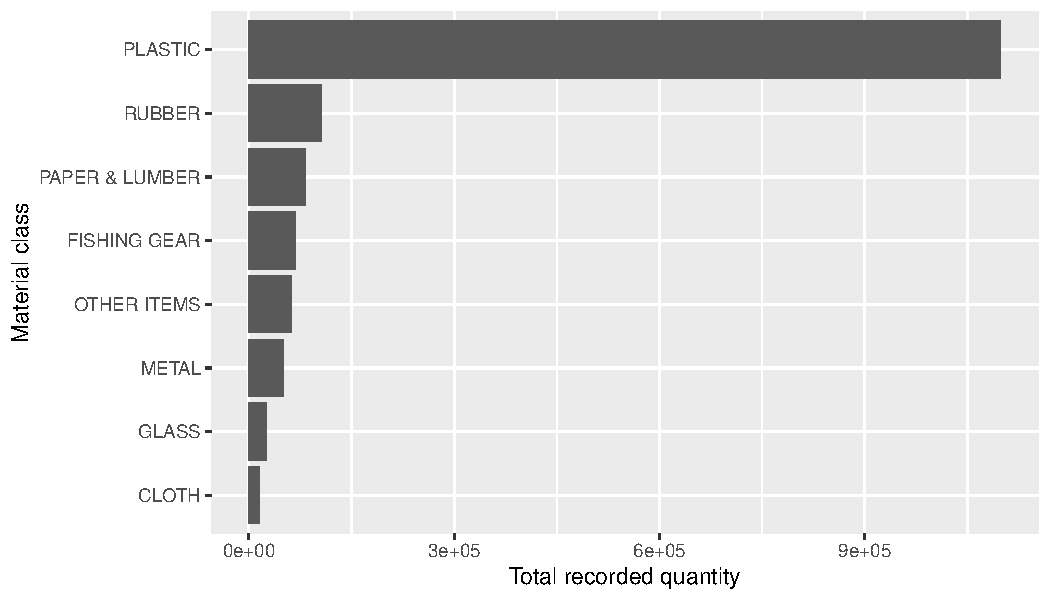
\includegraphics[width=\maxwidth]{figure/unnamed-chunk-11-1} 

\end{knitrout}
\caption {Material Quantities}
\label{figC}
\end {center}
\end {figure}

So the most populated material class is Plastic. Note that this does not necessarily mean that plastic is the largest quantity of debris, just that the individual number of items categorised is largest.

A tree map of material quantities:
\begin{figure}[H] %start a figure
\begin{center}

\caption {Debris categorisation}
\label{figI}
\end {center}
\end {figure}
\hl{chart disabled for now. This chart was working for a while (works in RStudio R, not LaTeX) only hint I can see is:\#\# Warning: Factor `ItemName` contains implicit NA, consider using `forcats::fct\_explicit\_na`}

Cigarettes are the most common item recorded as seen in. %Figure~\ref{figI}
Perhaps some of the debris is not actually from the sea, but rather from people littering by the coastline? Does debris littered on the coastline end up in the oceans?

\hl{This is a great chart, but not the best to support the statement that cigarettes is most popular - a column or bar chart here will be much better (area charts are not as effective as charts you can level-compare), potentially use proportions or data labels to further drive the point that it IS the largest. Treemap suggest moving back into pre-processing section.}



\subsection{Event-Driven Pollution}

Fireworks found in July and North-America only: possibly 4th July celebrations\\
4th July and Firework link? (Karen's Idea)\\

\begin{figure}[H] %start a figure
\begin{center}
\begin{knitrout}
\definecolor{shadecolor}{rgb}{0.969, 0.969, 0.969}\color{fgcolor}
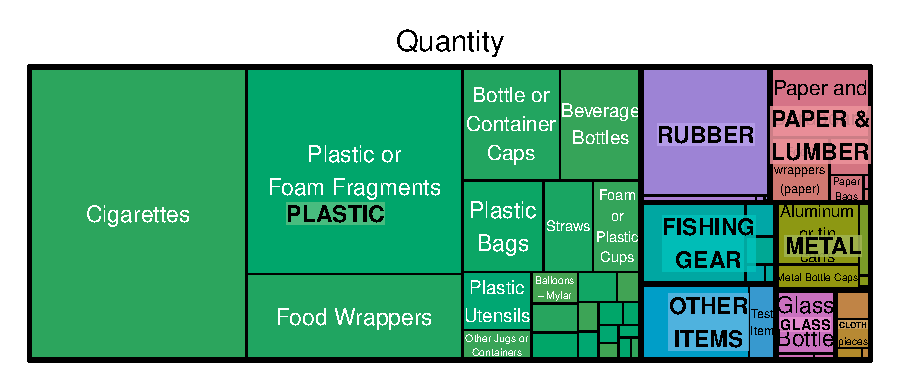
\includegraphics[width=\maxwidth]{figure/unnamed-chunk-13-1} 

\end{knitrout}

\caption {Boxplot of fireworks distribution by month, across all years}
\label{figA}
\end {center}
\end {figure}
\hl{this chart needs to size down}





\subsection{Location-Driven Pollution}

Rubber found in Indoneasia only: possibly a recording bias.\\

Certain classes are found in certain regions only: not because they don't exist elsewhere but because of recording bias focus in those areas\\

We have locational data, so lets check for any geographical observation bias.
\begin{knitrout}
\definecolor{shadecolor}{rgb}{0.969, 0.969, 0.969}\color{fgcolor}\begin{kframe}
\begin{alltt}
\hlstd{world} \hlkwb{<-} \hlkwd{map_data}\hlstd{(}\hlstr{"world"}\hlstd{)}
\hlstd{data} \hlopt
  \hlkwd{select}\hlstd{(Latitude, Longitude, Quantity, Location, `Material Description`)} \hlopt
  \hlkwd{ggplot}\hlstd{()} \hlopt{+}
    \hlkwd{geom_polygon}\hlstd{(}\hlkwc{data} \hlstd{=} \hlkwd{map_data}\hlstd{(}\hlstr{"world"}\hlstd{),} \hlkwd{aes}\hlstd{(}\hlkwc{x} \hlstd{= long,} \hlkwc{y} \hlstd{= lat,} \hlkwc{group} \hlstd{= group),} \hlkwc{fill} \hlstd{=} \hlstr{"grey"}\hlstd{,} \hlkwc{alpha} \hlstd{=} \hlnum{0.5}\hlstd{)} \hlopt{+}
    \hlkwd{geom_hex}\hlstd{(}\hlkwd{aes}\hlstd{(}\hlkwc{x} \hlstd{= Longitude,} \hlkwc{y} \hlstd{= Latitude),} \hlkwc{bins} \hlstd{=} \hlnum{50}\hlstd{)} \hlopt{+}
    \hlkwd{scale_fill_viridis}\hlstd{(}\hlkwc{trans} \hlstd{=} \hlstr{"log"}\hlstd{,} \hlkwc{breaks} \hlstd{=} \hlkwd{c}\hlstd{(}\hlnum{5}\hlstd{,} \hlnum{50}\hlstd{,} \hlnum{500}\hlstd{,} \hlnum{5000}\hlstd{,} \hlnum{50000}\hlstd{))} \hlopt{+}
    \hlkwd{theme_void}\hlstd{()} \hlopt{+}
    \hlkwd{guides}\hlstd{(}\hlkwc{fill}\hlstd{=}\hlkwd{guide_legend}\hlstd{(}\hlkwc{title}\hlstd{=}\hlstr{"Observations"}\hlstd{))}
\end{alltt}


{\ttfamily\noindent\color{warningcolor}{\#\# Warning: Computation failed in `stat\_binhex()`:\\\#\# Package `hexbin` required for `stat\_binhex`.\\\#\# Please install and try again.}}\end{kframe}
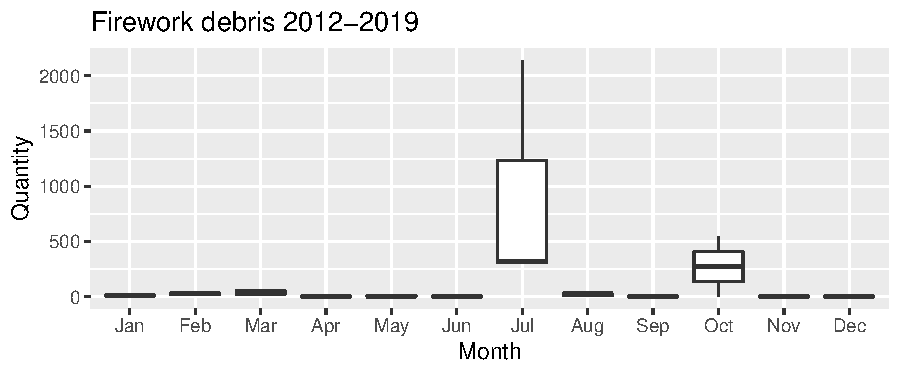
\includegraphics[width=\maxwidth]{figure/unnamed-chunk-14-1} 
\begin{kframe}\begin{alltt}
\hlcom{#ggsave("plots/map.png", width = 20, height = 10, units = "cm")}
\end{alltt}
\end{kframe}
\end{knitrout}
There seems to be a strong bias towards North America in our dataset. We will try a logarithmic plot to see things more clearly:
\begin{knitrout}
\definecolor{shadecolor}{rgb}{0.969, 0.969, 0.969}\color{fgcolor}\begin{kframe}
\begin{alltt}
\hlstd{data} \hlopt
  \hlkwd{select}\hlstd{(Latitude, Longitude, Quantity, Location, `Material Description`)} \hlopt
  \hlkwd{ggplot}\hlstd{()} \hlopt{+}
    \hlkwd{geom_polygon}\hlstd{(}\hlkwc{data} \hlstd{=} \hlkwd{map_data}\hlstd{(}\hlstr{"world"}\hlstd{),} \hlkwd{aes}\hlstd{(}\hlkwc{x} \hlstd{= long,} \hlkwc{y} \hlstd{= lat,} \hlkwc{group} \hlstd{= group),} \hlkwc{fill} \hlstd{=} \hlstr{"grey"}\hlstd{,} \hlkwc{alpha} \hlstd{=} \hlnum{0.5}\hlstd{)} \hlopt{+}
    \hlkwd{geom_hex}\hlstd{(}\hlkwd{aes}\hlstd{(}\hlkwc{x} \hlstd{= Longitude,} \hlkwc{y} \hlstd{= Latitude,} \hlkwc{fill} \hlstd{=} \hlkwd{stat}\hlstd{(}\hlkwd{log}\hlstd{(count))),} \hlkwc{bins} \hlstd{=} \hlnum{50}\hlstd{)} \hlopt{+}
    \hlkwd{scale_fill_viridis}\hlstd{()} \hlopt{+}
    \hlkwd{theme_void}\hlstd{()}
\end{alltt}


{\ttfamily\noindent\color{warningcolor}{\#\# Warning: Computation failed in `stat\_binhex()`:\\\#\# Package `hexbin` required for `stat\_binhex`.\\\#\# Please install and try again.}}\end{kframe}
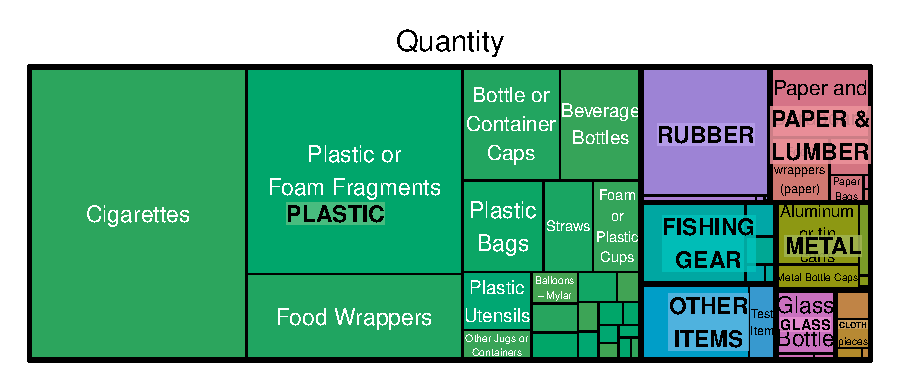
\includegraphics[width=\maxwidth]{figure/unnamed-chunk-15-1} 

\end{knitrout}

We need to know how reliable the location data is. I'm going to filter for "united kingdom" in the location field and plot the raw coordinates.\\

\begin{figure}[H] %start a figure
\begin{center}
\begin{knitrout}
\definecolor{shadecolor}{rgb}{0.969, 0.969, 0.969}\color{fgcolor}\begin{kframe}
\begin{alltt}
\hlcom{#Scatterplot of long/lat positions}
\hlstd{data} \hlopt
  \hlkwd{mutate}\hlstd{(}\hlkwc{Location} \hlstd{=} \hlkwd{str_to_lower}\hlstd{(Location))} \hlopt
  \hlkwd{filter}\hlstd{(}\hlkwd{str_detect}\hlstd{(Location,} \hlstr{"united kingdom"}\hlstd{))} \hlopt
  \hlkwd{select}\hlstd{(Latitude, Longitude)} \hlopt
  \hlkwd{ggplot}\hlstd{(}\hlkwd{aes}\hlstd{(}\hlkwc{x} \hlstd{= Latitude,} \hlkwc{y} \hlstd{= Longitude))} \hlopt{+}
    \hlkwd{geom_point}\hlstd{(}\hlkwc{position} \hlstd{=} \hlstr{"jitter"}\hlstd{)}
\end{alltt}
\end{kframe}
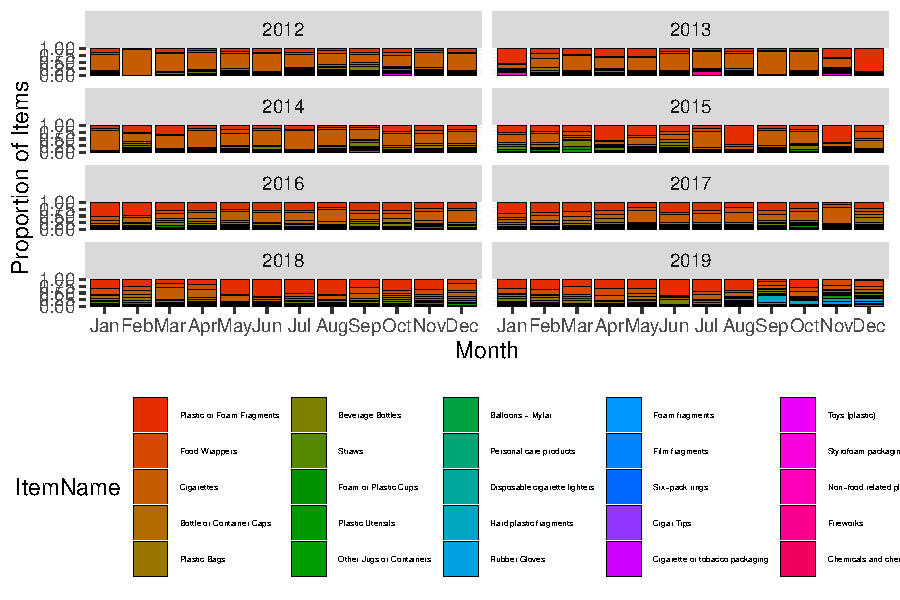
\includegraphics[width=\maxwidth]{figure/unnamed-chunk-16-1} 

\end{knitrout}
\caption {Longitude and Latitude discrepancies}
\label{figH}
\end {center}
\end {figure}
\hl{this chart needs to size down}
We have a outliers here. Maybe a difference in standards used for Longitude and Latitude? Some systems put the Latitude origin close to the UK.\\

Questions\\
Distribution of plastic by location.\\
Are the distributions of plastic fairly constant for the locations with the most observations?\\
\begin{figure}[H] %start a figure
\begin{center}
\begin{knitrout}
\definecolor{shadecolor}{rgb}{0.969, 0.969, 0.969}\color{fgcolor}
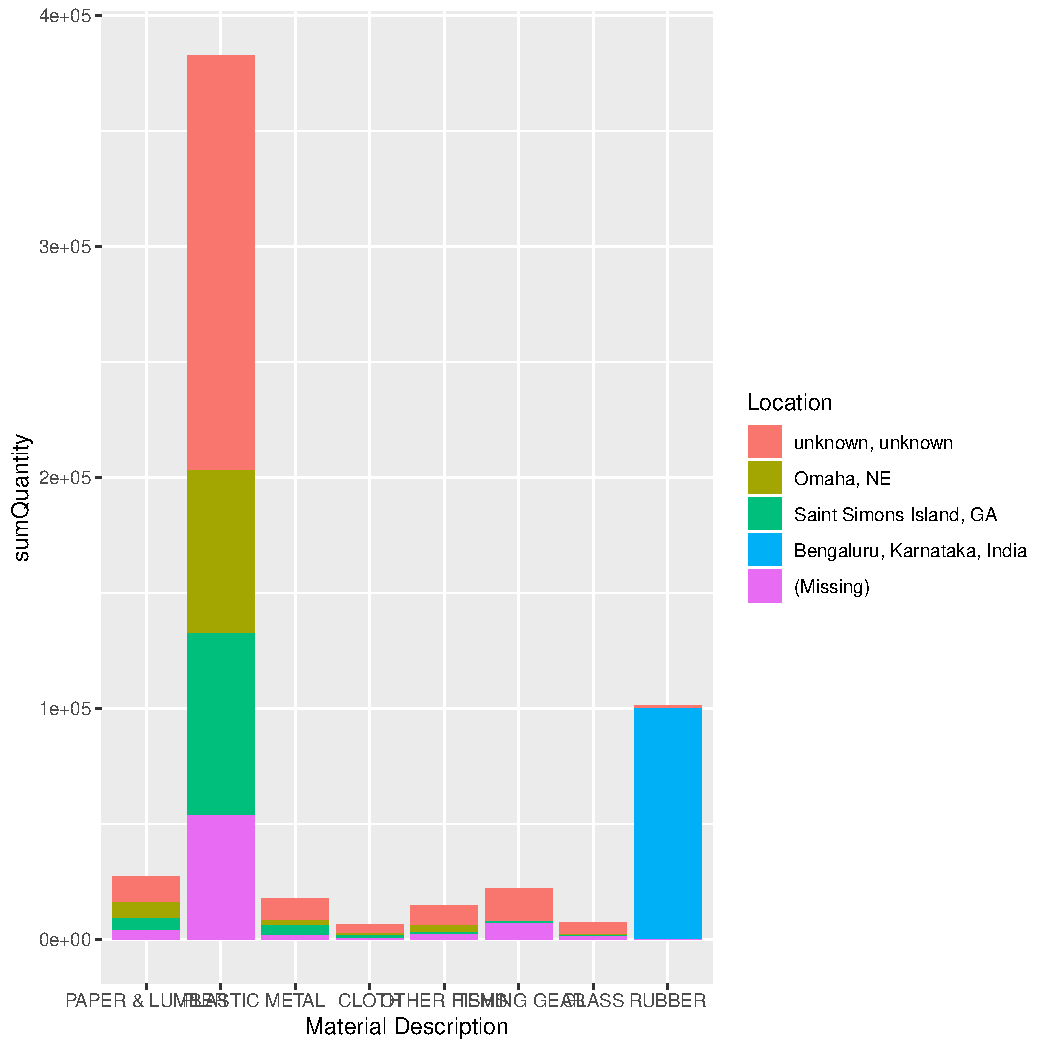
\includegraphics[width=\maxwidth]{figure/unnamed-chunk-17-1} 

\end{knitrout}
\caption {Debris by location}
\label{figG}
\end {center}
\end {figure}
We see that the Location "unknown" has the most plastic... note that this is distinct from "(Missing)", which was our original NA values. Maybe we should merge these.
\hl{this chart needs to size down}



\subsection{Item Pairing} 
(e.g. are 6-pack beer rings observed at the same time as fireworks? )
\hl{are we going to explore this one?}

\pagebreak
\section{Predictive Modelling}
The authors of this report built a model to predict the proportion of plastics given Month and Location. This would give more accurate predictions as opposed to a simple linear model, given we know that event-driven pollution will determine different pollutants are different times.

\subsection{Description of Model}

Georgios' script
\begin{knitrout}
\definecolor{shadecolor}{rgb}{0.969, 0.969, 0.969}\color{fgcolor}\begin{kframe}
\begin{alltt}
\hlstd{plasticN} \hlkwb{<-} \hlstd{plastic} \hlopt
  \hlkwd{mutate}\hlstd{(}\hlkwc{year} \hlstd{=} \hlkwd{as.integer}\hlstd{(}\hlkwd{year}\hlstd{(Time)))} \hlopt
  \hlkwd{filter}\hlstd{(year} \hlopt{>} \hlnum{2010}\hlstd{)} \hlopt
  \hlkwd{group_by}\hlstd{(year, category)} \hlopt
  \hlkwd{summarise}\hlstd{(}\hlkwc{`Total Quantity`} \hlstd{=} \hlkwd{sum}\hlstd{(Quantity))}

  \hlcom{####}
\hlkwd{library}\hlstd{(dplyr)}
\hlstd{df11N} \hlkwb{<-} \hlstd{plasticN}  \hlopt
  \hlkwd{filter}\hlstd{(year} \hlopt{==} \hlnum{2011}\hlstd{)} \hlopt
  \hlkwd{group_by}\hlstd{(year)} \hlopt
  \hlkwd{mutate}\hlstd{(}\hlkwc{freq} \hlstd{= `Total Quantity`} \hlopt{/} \hlkwd{sum}\hlstd{(`Total Quantity`))}

\hlstd{df12N} \hlkwb{<-} \hlstd{plasticN}  \hlopt
  \hlkwd{filter}\hlstd{(year} \hlopt{==} \hlnum{2012}\hlstd{)} \hlopt
  \hlkwd{group_by}\hlstd{(year)} \hlopt
  \hlkwd{mutate}\hlstd{(}\hlkwc{freq} \hlstd{= `Total Quantity`} \hlopt{/} \hlkwd{sum}\hlstd{(`Total Quantity`))}


\hlstd{df13N} \hlkwb{<-} \hlstd{plasticN}  \hlopt
  \hlkwd{filter}\hlstd{(year} \hlopt{==} \hlnum{2013}\hlstd{)} \hlopt
  \hlkwd{group_by}\hlstd{(year)} \hlopt
  \hlkwd{mutate}\hlstd{(}\hlkwc{freq} \hlstd{= `Total Quantity`} \hlopt{/} \hlkwd{sum}\hlstd{(`Total Quantity`))}


\hlstd{df14N} \hlkwb{<-} \hlstd{plasticN}  \hlopt
  \hlkwd{filter}\hlstd{(year} \hlopt{==} \hlnum{2014}\hlstd{)} \hlopt
  \hlkwd{group_by}\hlstd{(year)} \hlopt
  \hlkwd{mutate}\hlstd{(}\hlkwc{freq} \hlstd{= `Total Quantity`} \hlopt{/} \hlkwd{sum}\hlstd{(`Total Quantity`))}

\hlstd{df15N} \hlkwb{<-} \hlstd{plasticN}  \hlopt
  \hlkwd{filter}\hlstd{(year} \hlopt{==} \hlnum{2015}\hlstd{)} \hlopt
  \hlkwd{group_by}\hlstd{(year)} \hlopt
  \hlkwd{mutate}\hlstd{(}\hlkwc{freq} \hlstd{= `Total Quantity`} \hlopt{/} \hlkwd{sum}\hlstd{(`Total Quantity`))}


\hlstd{df16N} \hlkwb{<-} \hlstd{plasticN}  \hlopt
  \hlkwd{filter}\hlstd{(year} \hlopt{==} \hlnum{2016}\hlstd{)} \hlopt
  \hlkwd{group_by}\hlstd{(year)} \hlopt
  \hlkwd{mutate}\hlstd{(}\hlkwc{freq} \hlstd{= `Total Quantity`} \hlopt{/} \hlkwd{sum}\hlstd{(`Total Quantity`))}



\hlstd{df17N} \hlkwb{<-} \hlstd{plasticN}  \hlopt
  \hlkwd{filter}\hlstd{(year} \hlopt{==} \hlnum{2017}\hlstd{)} \hlopt
  \hlkwd{group_by}\hlstd{(year)} \hlopt
  \hlkwd{mutate}\hlstd{(}\hlkwc{freq} \hlstd{= `Total Quantity`} \hlopt{/} \hlkwd{sum}\hlstd{(`Total Quantity`))}


\hlstd{df18N} \hlkwb{<-} \hlstd{plasticN}  \hlopt
  \hlkwd{filter}\hlstd{(year} \hlopt{==} \hlnum{2018}\hlstd{)} \hlopt
  \hlkwd{group_by}\hlstd{(year)} \hlopt
  \hlkwd{mutate}\hlstd{(}\hlkwc{freq} \hlstd{= `Total Quantity`} \hlopt{/} \hlkwd{sum}\hlstd{(`Total Quantity`))}

\hlstd{df19N} \hlkwb{<-} \hlstd{plasticN}  \hlopt
  \hlkwd{filter}\hlstd{(year} \hlopt{==} \hlnum{2019}\hlstd{)} \hlopt
  \hlkwd{group_by}\hlstd{(year)} \hlopt
  \hlkwd{mutate}\hlstd{(}\hlkwc{freq} \hlstd{= `Total Quantity`} \hlopt{/} \hlkwd{sum}\hlstd{(`Total Quantity`))}


\hlstd{dfTotN} \hlkwb{<-} \hlkwd{rbind}\hlstd{(df11N, df12N, df13N, df14N, df15N, df16N, df17N, df18N, df19N)}

\hlcom{# plot for observing the data}
\hlstd{(time_plotfr2N} \hlkwb{<-} \hlkwd{ggplot}\hlstd{(dfTotN,} \hlkwd{aes}\hlstd{(}\hlkwc{x} \hlstd{= year,} \hlkwc{y} \hlstd{= freq,} \hlkwc{color}\hlstd{=category,} \hlkwc{fill} \hlstd{= category))} \hlopt{+}
  \hlkwd{geom_smooth}\hlstd{(}\hlkwc{method}\hlstd{=}\hlstr{"lm"}\hlstd{)} \hlopt{+}
  \hlkwd{geom_point}\hlstd{(}\hlkwc{size}\hlstd{=}\hlnum{3}\hlstd{)} \hlopt{+}
  \hlkwd{theme_bw}\hlstd{()} \hlopt{+}
  \hlkwd{xlab}\hlstd{(}\hlstr{"Years"}\hlstd{)} \hlopt{+}
  \hlkwd{ylab}\hlstd{(}\hlstr{"freq"}\hlstd{)} \hlopt{+}
  \hlkwd{ggtitle}\hlstd{(}\hlstr{"portion of plastic"}\hlstd{)} \hlopt{+}
  \hlkwd{expand_limits}\hlstd{(}\hlkwc{y}\hlstd{=}\hlnum{0}\hlstd{)} \hlopt{+}
  \hlkwd{scale_y_continuous}\hlstd{()} \hlopt{+}
  \hlkwd{scale_x_continuous}\hlstd{()}\hlopt{+}
  \hlkwd{theme}\hlstd{(}\hlkwc{legend.position}\hlstd{=}\hlstr{"bottom"}\hlstd{)}\hlopt{+}
  \hlkwd{theme}\hlstd{(}\hlkwc{legend.text} \hlstd{=} \hlkwd{element_text}\hlstd{(}\hlkwc{size}\hlstd{=}\hlnum{5}\hlstd{,} \hlkwc{face}\hlstd{=}\hlstr{"bold"}\hlstd{)))}

  \hlcom{### MODELING with new categorisation}


\hlcom{# create train and test set}
\hlstd{n} \hlkwb{<-} \hlkwd{nrow}\hlstd{(dfTotN)}  \hlcom{# Number of observations}
\hlstd{ntrain} \hlkwb{<-} \hlkwd{round}\hlstd{(n}\hlopt{*}\hlnum{0.75}\hlstd{)}  \hlcom{# 75% for training set}
\hlkwd{set.seed}\hlstd{(}\hlnum{314}\hlstd{)}    \hlcom{# Set seed for reproducible results}
\hlstd{tindex} \hlkwb{<-} \hlkwd{sample}\hlstd{(n, ntrain)}   \hlcom{# Create a random index}
\hlstd{train_dfTotN} \hlkwb{<-} \hlstd{dfTotN[tindex,]}   \hlcom{# Create training set}
\hlstd{test_dfTotN} \hlkwb{<-} \hlstd{dfTotN[}\hlopt{-}\hlstd{tindex,]}

\hlcom{#  Pr(>|t|) is the p-value, defined as the probability of observing any value equal or larger than t if H0 is true. The larger the t statistic, the smaller the p-value. Generally, we use 0.05 as the cutoff for significance; when p-values are smaller than 0.05, we reject H0. Here p is pretty big which means that there is statistically significant correlation between relative frequency and years passing by. Which basically further supports our initial hypothesis in this project. I have included a prediction on the test set but it is of no worth obviously.}


\hlcom{# linear model on train set}
\hlkwd{print}\hlstd{(}\hlstr{"train model"}\hlstd{)}
\hlkwd{set.seed}\hlstd{(}\hlnum{1234}\hlstd{)}
\hlstd{dfTot_train.modelN} \hlkwb{<-} \hlkwd{lm}\hlstd{(freq} \hlopt{~} \hlstd{year,} \hlkwc{data} \hlstd{= train_dfTotN)}
\hlkwd{summary}\hlstd{(dfTot_train.modelN)}

\hlcom{# plotting frequencies according to train data}
\hlkwd{ggplot}\hlstd{(}\hlkwc{data} \hlstd{= train_dfTotN,} \hlkwd{aes}\hlstd{(}\hlkwc{x} \hlstd{= year,} \hlkwc{y} \hlstd{= freq))} \hlopt{+}
\hlkwd{geom_point}\hlstd{()} \hlopt{+}
\hlkwd{stat_smooth}\hlstd{(}\hlkwc{method} \hlstd{=} \hlstr{"lm"}\hlstd{,} \hlkwc{col} \hlstd{=} \hlstr{"dodgerblue3"}\hlstd{)} \hlopt{+}
\hlkwd{theme}\hlstd{(}\hlkwc{panel.background} \hlstd{=} \hlkwd{element_rect}\hlstd{(}\hlkwc{fill} \hlstd{=} \hlstr{"white"}\hlstd{),}
\hlkwc{axis.line.x}\hlstd{=}\hlkwd{element_line}\hlstd{(),}
\hlkwc{axis.line.y}\hlstd{=}\hlkwd{element_line}\hlstd{())} \hlopt{+}
\hlkwd{ggtitle}\hlstd{(}\hlstr{"Linear Model Fitted to Data"}\hlstd{)}


\hlkwd{print}\hlstd{(}\hlstr{"PREDICTION"}\hlstd{)}
\hlstd{predN} \hlkwb{<-} \hlkwd{predict}\hlstd{(dfTot_train.modelN, test_dfTotN)}
\hlkwd{summary}\hlstd{(predN)}

\hlcom{# make actuals_predicteds dataframe}
\hlstd{actuals_preds} \hlkwb{<-} \hlkwd{data.frame}\hlstd{(}\hlkwd{cbind}\hlstd{(}\hlkwc{actuals}\hlstd{=test_dfTotN}\hlopt{$}\hlstd{freq,} \hlkwc{predicteds}\hlstd{=predN))}
\hlkwd{head}\hlstd{(actuals_preds)}
\hlcom{# A simple correlation between the actuals and predicted values can be used as a form of accuracy measure. A higher correlation accuracy implies that the actuals and predicted values have similar directional movement, i.e. when the actuals values increase the predicteds also increase and vice-versa.}

\hlstd{correlation_accuracy} \hlkwb{<-} \hlkwd{cor}\hlstd{(actuals_preds)}  \hlcom{# 5.31%}
\hlstd{min_max_accuracy} \hlkwb{<-} \hlkwd{mean}\hlstd{(}\hlkwd{apply}\hlstd{(actuals_preds,} \hlnum{1}\hlstd{, min)} \hlopt{/} \hlkwd{apply}\hlstd{(actuals_preds,} \hlnum{1}\hlstd{, max))}
\hlcom{# => 53.73%, min_max accuracy}
\hlstd{mape} \hlkwb{<-} \hlkwd{mean}\hlstd{(}\hlkwd{abs}\hlstd{((actuals_preds}\hlopt{$}\hlstd{predicteds} \hlopt{-} \hlstd{actuals_preds}\hlopt{$}\hlstd{actuals))}\hlopt{/}\hlstd{actuals_preds}\hlopt{$}\hlstd{actuals)}
\hlcom{# => 99.4%, mean absolute percentage deviation}
\hlcom{# Intrestingly enough min_max accuracy and mostly mean absolute percentage deviation score quite well}
\hlcom{# but still on a model that can not be trusted.}
\end{alltt}
\end{kframe}
\end{knitrout}

\subsection{Model Evaluation}


\subsection{Model Results}
Time does not impact plastic composition.

\pagebreak
\section{Discussion}



\section{Conclusion and Future Work}\label{cdsmote1}

Our hypothesis stands/does not stand.


%Edit here 
%\blindtext[2]




\pagebreak
\section{Project Management}\label{mgt}
\subsection{Facilities}
Group 2 communicated using a dedicated Slack Channel, Github repository and weekly 1 hour meetings before the wednesday lab.
All project documents used and the final report can be accessed from the \textit{\href{https://github.com/KarenJewell/CMM507Group2}{Public Github Repository}}
\hl{obviously we need to mention the whole covid-19 thing and how we worked around it.}

\subsection{Project Progress}

% Pay attention to the code below including the chunk options 
% latex table generated in R 3.6.1 by xtable 1.8-4 package
% Mon Apr 13 21:57:25 2020
\begin{table}[ht]
\centering
\caption{Record of Team Meetings} 
\label{tab:one}
\begin{tabular}{llp{8cm}lllll}
  \hline
No & Date & Topic & Alex & Georgios & Karen & Roshi & Stuart \\ 
  \hline
1.00 & 2020-02-05 & Group Formation: set up communication channel in Slack and GitHub repository & yes & yes & yes & yes & yes \\ 
  2.00 & 2020-02-11 & Agreed topic of "Plastic Pollution", distributed research activity for week & yes & yes & yes & yes & yes \\ 
  3.00 & 2020-02-18 & Presented inividuals' research findings and discussed hypothesis & yes & yes & yes & yes & yes \\ 
  4.00 & 2020-02-25 & Decided on final dataset to use and hypothesis of "proportion of marine plastics pollution does not change over time" & yes & yes & yes & yes & yes \\ 
  5.00 & 2020-03-04 & Presentation draft agreed & yes & yes & yes & yes & yes \\ 
  6.00 & 2020-03-10 & Distributed section writing activity for week & yes & yes & yes & yes & yes \\ 
  7.00 & 2020-03-17 &  &  &  &  &  &  \\ 
  8.00 & 2020-03-24 &  &  &  &  &  &  \\ 
  9.00 & 2020-03-31 &  &  &  &  &  &  \\ 
  10.00 & 2020-04-07 &  &  &  &  &  &  \\ 
  11.00 & 2020-04-14 &  &  &  &  &  &  \\ 
  12.00 & 2020-04-21 &  &  &  &  &  &  \\ 
   \hline
\end{tabular}
\end{table}





\subsection{Peer-assessment}

% latex table generated in R 3.6.1 by xtable 1.8-4 package
% Mon Apr 13 21:57:26 2020
\begin{table}[ht]
\centering
\caption{Peer Assessment out of 100} 
\label{tab:two}
\begin{tabular}{llllll}
  \hline
Peer.Review & Alex & Georgios & Karen & Roshi & Stuart \\ 
  \hline
Alex & 100 & 100 & 100 & 100 & 100 \\ 
  Georgios & 100 & 100 & 100 & 100 & 100 \\ 
  Karen & 100 & 100 & 100 & 100 & 100 \\ 
  Roshi & 100 & 100 & 100 & 100 & 100 \\ 
  Stuart & 100 & 100 & 100 & 100 & 100 \\ 
   \hline
\end{tabular}
\end{table}



\pagebreak
\section*{References}\label{pubs}
\printbibliography[heading =none]

\end{document}
